% Here we import all packages and set the document type
\documentclass[12pt,spanish,fleqn,openany,letterpaper,pagesize]{scrbook}

\usepackage[utf8]{inputenc}
\usepackage[spanish]{babel}
\usepackage{fancyhdr}
\usepackage{epsfig}
\usepackage{epic}
\usepackage{eepic}
\usepackage{amsmath}
\usepackage{threeparttable}
\usepackage{amscd}
\usepackage{here}
\usepackage{graphicx}
\usepackage{lscape}
\usepackage{tabularx}
\usepackage{subfigure}
\usepackage{longtable}


\usepackage{rotating} %Para rotar texto, objetos y tablas seite. No se ve en DVI solo en PS. Seite 328 Hundebuch
                        %se usa junto con \rotate, \sidewidestable ....


\renewcommand{\theequation}{\thechapter-\arabic{equation}}
\renewcommand{\thefigure}{\textbf{\thechapter-\arabic{figure}}}
\renewcommand{\thetable}{\textbf{\thechapter-\arabic{table}}}


\pagestyle{fancyplain}%\addtolength{\headwidth}{\marginparwidth}
\textheight22.5cm \topmargin0cm \textwidth16.5cm
\oddsidemargin0.5cm \evensidemargin-0.5cm%
\renewcommand{\chaptermark}[1]{\markboth{\thechapter\; #1}{}}
\renewcommand{\sectionmark}[1]{\markright{\thesection\; #1}}
\lhead[\fancyplain{}{\thepage}]{\fancyplain{}{\rightmark}}
\rhead[\fancyplain{}{\leftmark}]{\fancyplain{}{\thepage}}
\fancyfoot{}
\thispagestyle{fancy}%


\addtolength{\headwidth}{0cm}
\unitlength1mm %Define la unidad LE para Figuras
\mathindent0cm %Define la distancia de las formulas al texto,  fleqn las descentra
\marginparwidth0cm
\parindent0cm %Define la distancia de la primera linea de un parrafo a la margen

%Para tablas,  redefine el backschlash en tablas donde se define la posici\'{o}n del texto en las
%casillas (con \centering \raggedright o \raggedleft)
\newcommand{\PreserveBackslash}[1]{\let\temp=\\#1\let\\=\temp}
\let\PBS=\PreserveBackslash

%Espacio entre lineas
\renewcommand{\baselinestretch}{1.1}

%Neuer Befehl f\"{u}r die Tabelle Eigenschaften der Aktivkohlen
\newcommand{\arr}[1]{\raisebox{1.5ex}[0cm][0cm]{#1}}

%Neue Kommandos
\usepackage{Befehle}


%Trennungsliste
\hyphenation {Reaktor-ab-me-ssun-gen Gas-zu-sa-mmen-set-zung
Raum-gesch-win-dig-keit Durch-fluss Stick-stoff-gemisch
Ad-sorp-tions-tem-pe-ra-tur Klein-schmidt
Kohlen-stoff-Mole-kular-siebe Py-rolysat-aus-beu-te
Trans-port-vor-gan-ge}

%\includeonly{Kap1/Kap1,Kap2/Kap2}
\begin{document}

\pagenumbering{roman}

%\newpage
%\setcounter{page}{1}
\begin{center}
\begin{figure}
\centering%

\epsfig{file=HojaTitulo/logoFAMAF.jpg,scale=0.8}%
\end{figure}
\thispagestyle{empty} \vspace*{0.1cm} \textbf{\huge
Estratificación temporal de Aedes Aegypti basada en herramientas geoespaciales y aprendizaje automático}\\[9.0cm]
\Large\textbf{Juan Manuel Scavuzzo}\\[0.5cm]
\small Universidad Nacional de Córdoba\\
Facultad de Matemática, Astronomía, Física y Computación\\
Córdoba, Argentina\\
2018\\
\end{center}

\newpage{\pagestyle{empty}\cleardoublepage}

\newpage
\begin{center}
\thispagestyle{empty} \vspace*{0cm} \textbf{\huge
Estratificación temporal de Aedes Aegypti basada en herramientas Geoespaciales y Machine Learning}\\[3.0cm]
\Large\textbf{Juan Manuel Scavuzzo}\\[2.0cm]
\small Tesis de grado presentada como requisito parcial para optar al
título de:\\
\textbf{Licenciado en Ciencias de la Computación}\\[2.5cm]
Directores:\\

Mgter. Gonzalo Sebastián Peralta (Licenciado en Cs de la Computación y Magíster en Aplicaciones Espaciales)\\
Dr. Jorge Sánchez (Ingeniero en Electrónica y Doctor en Ciencias de la Ingeniería, Visión por computadoras y reconocimiento de patrones)\\ [3.0cm]

Universidad Nacional de Córdoba\\
Facultad de Matemática, Astronomía, Física y Computación\\
Córdoba, Argentina\\
2018\\\end{center}

\newpage{\pagestyle{empty}\cleardoublepage}

\newpage
\thispagestyle{empty} \textbf{}\normalsize
\\\\\\%
\textbf{(Dedicatoria o un lema)}\\[4.0cm]

\begin{flushright}
\begin{minipage}{8cm}
    \noindent
        \small
        Aca va algun lema o algo asi
        Por ejemplo:\\[1.0cm]
        A mis padres\\[1.0cm]\\
        o\\[1.0cm]
        La preocupaci\'{o}n por el hombre y su destino siempre debe ser el
        inter\'{e}s primordial de todo esfuerzo t\'{e}cnico. Nunca olvides esto
        entre tus diagramas y ecuaciones.\\\\
        Albert Einstein\\
\end{minipage}
\end{flushright}

\newpage{\pagestyle{empty}\cleardoublepage}

\newpage
\thispagestyle{empty} \textbf{}\normalsize
\\\\\\%
\textbf{\LARGE Agradecimientos}
\addcontentsline{toc}{chapter}{\numberline{}Agradecimientos}\\\\
insertar agradecimientos

\newpage{\pagestyle{empty}\cleardoublepage}

\newpage
\textbf{\LARGE Resumen}
\addcontentsline{toc}{chapter}{\numberline{}Resumen}\\\\

\textbf{\small Palabras clave: Computer Science, Machine Learning, Python,
      Landscape Epidemiology, Remote Sensing, Dengue, Zika, Chikungunya, Public Health}.\\
\justifying
  \par El Dengue, Zika y Chikungunya son enfermedades virales cuya vacuna para
    prevención aún no existe y que, en los últimos años, han tenido un incremento
    e impacto en la población de la región argentina y latinoamericana que ha
    sido de gran preocupación para los organismos gubernamentales de salud.

  \par En los últimos años se han generado sistemas de riesgo de transmisión
    de enfermedades virales basados en información de sensores remotos,
    estableciendo relaciones entre las condiciones ambientales de las distintas
    zonas con la abundancia del vector en las mismas. A dicha área de estudio
    se la denomina Epidemiología Panorámica.

 \par En el presente trabajo, por un lado, utilizando técnicas de
    ingeniería del software para extraer los requerimientos y aplicar una metodología
    de desarrollo acorde a las necesidades,
    se implementa un \textit{framework} para la generación de modelos de
    aprendizaje automático (ML) con el objetivo
    de estimar la abundancia de vectores de Dengue, Zika y Chikungunya.
    A su vez, se entrenan y evalúan modelos no lineales que poseen mayor
    capacidad de generalización a la hora de modelar las poblaciones del
    mosquito, en comparación con los modelos que actualmente se utilizan
    para tal fin.

  \par Se presenta, además, un enfoque que resuelve el problema de que
    un modelo entrenado con información de una sola ciudad no es capaz,
    en principio, de estimar correctamente la abudancia en otras zonas del país.
    En este trabajo
    se propone resolver la cuestión a traves de un concepto novedoso en el campo
    de la epidemiología, que establece
    relaciones de ``cercanía``
    entre regiones teniendo en cuenta sus características
    ambientales: la Distancia Ambiental Normalizada.


\renewcommand{\tablename}{\textbf{Tabla}}
\renewcommand{\figurename}{\textbf{Figura}}
\renewcommand{\listtablename}{Lista de Tablas}
\renewcommand{\listfigurename}{Lista de Figuras}
\renewcommand{\contentsname}{Contenido}


%\newcommand{\clearemptydoublepage}{\newpage{\pagestyle{empty}\cleardoublepage}}
\tableofcontents
%\include{Resumen}%\newcommand{\clearemptydoublepage}{\newpage{\pagestyle{empty}\cleardoublepage}}
\pagenumbering{arabic}
\chapter{Introducci\'{o}n}
En la introducci\'{o}n, el autor presenta y se\~{n}ala la importancia, el origen (los antecedentes te\'{o}ricos y pr\'{a}cticos), los objetivos, los alcances, las limitaciones, la metodolog\'{\i}a empleada, el significado que el estudio tiene en el avance del campo respectivo y su aplicaci\'{o}n en el \'{a}rea investigada. No debe confundirse con el resumen y se recomienda que la introducci\'{o}n tenga una extensi\'{o}n de m\'{\i}nimo 2 p\'{a}ginas y m\'{a}ximo de 4 p\'{a}ginas.\\

La presente plantilla maneja una familia de fuentes utilizada generalmente en LaTeX, conocida como Computer Modern, espec\'{\i}ficamente LMRomanM para el texto de los p\'{a}rrafos y CMU Sans Serif para los t\'{\i}tulos y subt\'{\i}tulos. Sin embargo, es posible sugerir otras fuentes tales como Garomond, Calibri, Cambria, Arial o Times New Roman, que por claridad y forma, son adecuadas para la edici\'{o}n de textos acad\'{e}micos.\\

La presente plantilla tiene en cuenta aspectos importantes de la Norma T\'{e}cnica Colombiana - NTC 1486, con el fin que sea usada para la presentaci\'{o}n final de las tesis de maestr\'{\i}a y doctorado y especializaciones y especialidades en el \'{a}rea de la salud, desarrolladas en la Universidad Nacional de Colombia.\\

Las m\'{a}rgenes, numeraci\'{o}n, tama\~{n}o de las fuentes y dem\'{a}s aspectos de formato, deben ser conservada de acuerdo con esta plantilla, la cual esta dise\~{n}ada para imprimir por lado y lado en hojas tama\~{n}o carta. Se sugiere que los encabezados cambien seg\'{u}n la secci\'{o}n del documento (para lo cual esta plantilla esta construida por secciones).\\

Si se requiere ampliar la informaci\'{o}n sobre normas adicionales para la escritura se puede consultar la norma NTC 1486 en la Base de datos del ICONTEC (Normas T\'{e}cnicas Colombianas) disponible en el portal del SINAB de la Universidad Nacional de Colombia\footnote{ver: www.sinab.unal.edu.co}, en la secci\'{o}n "Recursos bibliogr\'{a}ficos" opci\'{o}n "Bases de datos".  Este portal tambi\'{e}n brinda la posibilidad de acceder a un instructivo para la utilizaci\'{o}n de Microsoft Word y Acrobat Professional, el cual est\'{a} disponible en la secci\'{o}n "Servicios", opci\'{o}n "Tr\'{a}mites" y enlace "Entrega de tesis".\\

La redacci\'{o}n debe ser impersonal y gen\'{e}rica. La numeraci\'{o}n de las hojas sugiere que las p\'{a}ginas preliminares se realicen en n\'{u}meros romanos en may\'{u}scula y las dem\'{a}s en n\'{u}meros ar\'{a}bigos, en forma consecutiva a partir de la introducci\'{o}n que comenzar\'{a} con el n\'{u}mero 1. La cubierta y la portada no se numeran pero si se cuentan como p\'{a}ginas.\\

Para trabajos muy extensos se recomienda publicar m\'{a}s de un volumen. Se debe tener en cuenta que algunas facultades tienen reglamentada la extensi\'{o}n m\'{a}xima de las tesis  o trabajo de investigaci\'{o}n; en caso que no sea as\'{\i}, se sugiere que el documento no supere 120 p\'{a}ginas.\\

No se debe utilizar numeraci\'{o}n compuesta como 13A, 14B \'{o} 17 bis, entre otros, que indican superposici\'{o}n de texto en el documento. Para resaltar, puede usarse letra cursiva o negrilla. Los t\'{e}rminos de otras lenguas que aparezcan dentro del texto se escriben en cursiva.\\
\chapter{Cap\'{\i}tulo 1}
Los cap\'{\i}tulos son las principales divisiones del documento. En estos, se desarrolla el tema del documento. Cada cap\'{\i}tulo debe corresponder a uno de los temas o aspectos tratados en el documento y por tanto debe llevar un t\'{\i}tulo que indique el contenido del cap\'{\i}tulo.\\

Los t\'{\i}tulos de los cap\'{\i}tulos deben ser concertados entre el alumno y el director de la tesis  o trabajo de investigaci\'{o}n, teniendo en cuenta los lineamientos que cada unidad acad\'{e}mica brinda. As\'{\i} por ejemplo, en algunas facultades se especifica que cada cap\'{\i}tulo debe corresponder a un art\'{\i}culo cient\'{\i}fico, de tal manera que se pueda publicar posteriormente en una revista.\\

\section{Subt\'{\i}tulos nivel 2}
Toda divisi\'{o}n o cap\'{\i}tulo, a su vez, puede subdividirse en otros niveles y s\'{o}lo se enumera hasta el tercer nivel. Los t\'{\i}tulos de segundo nivel se escriben con min\'{u}scula al margen izquierdo y sin punto final, est\'{a}n separados del texto o contenido por un interlineado posterior de 10 puntos y anterior de 20 puntos (tal y como se presenta en la plantilla).\\

\subsection{Subt\'{\i}tulos nivel 3}
De la cuarta subdivisi\'{o}n en adelante, cada nueva divisi\'{o}n o \'{\i}tem puede ser se\~{n}alada con vi\~{n}etas, conservando el mismo estilo de \'{e}sta, a lo largo de todo el documento.\\

Las subdivisiones, las vi\~{n}etas y sus textos acompa\~{n}antes deben presentarse sin sangr\'{\i}a y justificados.\\

\begin{itemize}
\item En caso que sea necesario utilizar vi\~{n}etas, use este formato (vi\~{n}etas cuadradas).
\end{itemize}
\chapter{Cap\'{\i}tulo 2}
Existen varias normas para la citaci\'{o}n bibliogr\'{a}fica. Algunas \'{a}reas del conocimiento prefieren normas espec\'{\i}ficas para citar las referencias bibliogr\'{a}ficas en el texto y escribir la lista de bibliograf\'{\i}a al final de los documentos. Esta plantilla brinda la libertad para que el autor de la tesis  o trabajo de investigaci\'{o}n utilice la norma bibliogr\'{a}fica com\'{u}n para su disciplina. Sin embargo, se solicita que la norma seleccionada se utilice con rigurosidad, sin olvidar referenciar "todos" los elementos tomados de otras fuentes (referencias bibliogr\'{a}ficas, patentes consultadas, software empleado en el manuscrito, en el tratamiento a los datos y resultados del trabajo, consultas a personas (expertos o p\'{u}blico general), entre otros).\\

\section{Ejemplos de citaciones bibliogr\'{a}ficas}
Existen algunos ejemplos para la citaci\'{o}n bibliogr\'{a}fica, por ejemplo, Microsoft Word (versiones posteriores al 2006), en el  men\'{u} de referencias, se cuenta con la opci\'{o}n de insertar citas bibliogr\'{a}ficas utilizando la norma APA (American Psychological Association) u otras normas y con la ayuda para construir autom\'{a}ticamente la lista al final del documento. De la misma manera, existen administradores bibliogr\'{a}ficos compatibles con Microsoft Word como Zotero, End Note y el Reference Manager,  disponibles a trav\'{e}s del Sistema Nacional de Bibliotecas (SINAB) de la Universidad Nacional de Colombia\footnote{Ver:www.sinab.unal.edu.co } secci\'{o}n "Recursos bibliogr\'{a}ficos" opci\'{o}n "Herramientas Bibliogr\'{a}ficas. A continuaci\'{o}n se muestra un ejemplo de una de las formas m\'{a}s usadas para las citaciones bibliogr\'{a}ficas.\\

Citaci\'{o}n individual:\cite{AG01}.\\
Citaci\'{o}n simult\'{a}nea de varios autores:
\cite{AG12,AG52,AG70,AG08a,AG09a,AG36a,AG01i}.\\

Por lo general, las referencias bibliogr\'{a}ficas correspondientes a los anteriores n\'{u}meros, se listan al final del documento en orden de aparici\'{o}n o en orden alfab\'{e}tico. Otras normas de citaci\'{o}n incluyen el apellido del autor y el a\~{n}o de la referencia, por ejemplo: 1) "...\'{e}nfasis en elementos ligados al \'{a}mbito ingenieril que se enfocan en el manejo de datos e informaci\'{o}n estructurada y que seg\'{u}n Kostoff (1997) ha atra\'{\i}do la atenci\'{o}n de investigadores dado el advenimiento de TIC...", 2) "...Dicha afirmaci\'{o}n coincide con los planteamientos de Snarch (1998), citado por Castellanos (2007), quien comenta que el manejo..." y 3) "...el futuro del sistema para argumentar los procesos de toma de decisiones y el desarrollo de ideas innovadoras (Nosella \textsl{et al}., 2008)...".\\

\section{Ejemplos de presentaci\'{o}n y citaci\'{o}n de figuras}
Las ilustraciones forman parte del contenido de los cap\'{\i}tulos. Se deben colocar en la misma p\'{a}gina en que se mencionan o en la siguiente (deben siempre mencionarse en el texto).\\

Las llamadas para explicar alg\'{u}n aspecto de la informaci\'{o}n deben hacerse con nota al pie y su nota correspondiente\footnote{Las notas van como "notas al pie". Se utilizan para explicar, comentar o hacer referencia al texto de un documento, as\'{\i} como para introducir comentarios detallados y en ocasiones para citar fuentes de informaci\'{o}n (aunque para esta opci\'{o}n es mejor seguir en detalle las normas de citaci\'{o}n bibliogr\'{a}fica seleccionadas).}. La fuente documental se debe escribir al final de la ilustraci\'{o}n o figura con los elementos de la referencia (de acuerdo con las normas seleccionadas) y no como pie de p\'{a}gina. Un ejemplo para la presentaci\'{o}n y citaci\'{o}n de figuras, se presenta a continuaci\'{o}n (citaci\'{o}n directa):\\

Por medio de las propiedades del fruto, seg\'{u}n el espesor del endocarpio, se hace una clasificaci\'{o}n de la palma de aceite en tres tipos: Dura, Ternera y Pisifera, que se ilustran en la Figura
\ref{fig:Fruto}.\\
\begin{figure}
\centering%
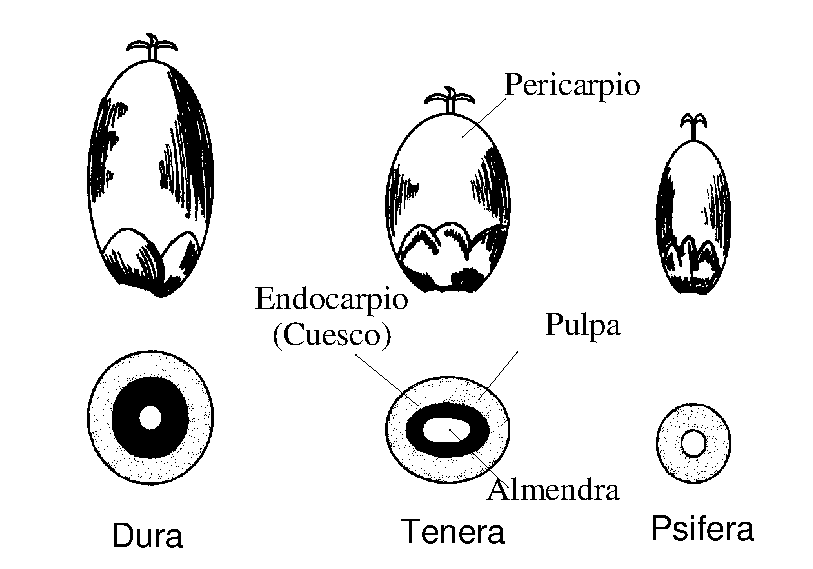
\includegraphics{Cap3/FrutoSp}%
\caption{Tipos y partes del fruto de palma de aceite \cite{AG03p,AG04p}.} \label{fig:Fruto}
\end{figure}

\section{Ejemplo de presentaci\'{o}n y citaci\'{o}n de tablas y cuadros}
Para la edici\'{o}n de tablas, cada columna debe llevar su t\'{\i}tulo; la primera palabra se debe escribir con may\'{u}scula inicial y preferiblemente sin abreviaturas. En las tablas y cuadros, los t\'{\i}tulos y datos se deben ubicar entre l\'{\i}neas horizontales y verticales cerradas (como se realiza en esta plantilla).\\

La numeraci\'{o}n de las tablas se realiza de la misma manera que las figuras o ilustraciones, a lo largo de todo el texto. Deben llevar un t\'{\i}tulo breve, que concreta el contenido de la tabla; \'{e}ste se debe escribir en la parte superior de la misma. Para la presentaci\'{o}n de cuadros, se deben seguir las indicaciones dadas para las tablas.\\

Un ejemplo para la presentaci\'{o}n y citaci\'{o}n de tablas (citaci\'{o}n indirecta), se presenta a continuaci\'{o}n:\\

De esta participaci\'{o}n aproximadamente el 60 \% proviene de biomasa
(Tabla \ref{EMundo1}).
\begin{center}
\begin{threeparttable}
\centering%
\caption{Participaci\'{o}n de las energ\'{\i}as renovables en el suministro
total de energ\'{\i}a primaria \cite{AG02i}.}\label{EMundo1}
\begin{tabular}{|l|c|c|}\hline
&\multicolumn{2}{c|}{Participaci\'{o}n en el suministro de energ\'{\i}a primaria /\% (Mtoe)\;$\tnote{1}$}\\\cline{2-3}%
\arr{Region}&Energ\'{\i}as renovables &Participaci\'{o}n de la biomasa\\\hline%
Latinoam\'{e}rica&28,9 (140)&62,4 (87,4)\\\hline%
\:Colombia&27,7 (7,6)&54,4 (4,1)\\\hline%
Alemania&3,8 (13,2)&65,8 (8,7)\\\hline%
Mundial&13,1 (1404,0)&79,4 (1114,8)\\\hline
\end{tabular}
\begin{tablenotes}
\item[1] \footnotesize{1 kg oe=10000 kcal=41,868 MJ}
\end{tablenotes}
\end{threeparttable}
\end{center}

NOTA: en el caso en que el contenido de la tabla o cuadro sea muy extenso, se puede cambiar el tama\~{n}o de la letra, siempre y cuando \'{e}sta sea visible por el lector.\\

\subsection{Consideraciones adicionales para el manejo de figuras y tablas}
Cuando una tabla, cuadro o figura ocupa m\'{a}s de una p\'{a}gina, se debe repetir su identificaci\'{o}n num\'{e}rica, seguida por la palabra continuaci\'{o}n.\\

Adicionalmente los encabezados de las columnas se deben repetir en todas las p\'{a}ginas despu\'{e}s de la primera.\\

Los anteriores lineamientos se contemplan en la presente plantilla.\\

\begin{itemize}
\item Presentaci\'{o}n y citaci\'{o}n de ecuaciones.
\end{itemize}

La citaci\'{o}n de ecuaciones, en caso que se presenten, debe hacerse como lo sugiere esta plantilla. Todas las ecuaciones deben estar numeradas y citadas detro del texto.\\

Para el manejo de cifras se debe seleccionar la norma seg\'{u}n el \'{a}rea de conocimiento de la tesis  o trabajo de investigaci\'{o}n.\\

\chapter{Cap\'{\i}tulo 3}
Se deben incluir tantos cap\'{\i}tulos como se requieran; sin embargo, se recomienda que la tesis  o trabajo de investigaci\'{o}n tenga un m\'{\i}nimo 3 cap\'{\i}tulos y m\'{a}ximo de 6 cap\'{\i}tulos (incluyendo las conclusiones).\\
\chapter{Cap\'{\i}tulo ...}
Se deben incluir tantos cap\'{\i}tulos como se requieran; sin embargo, se recomienda que la tesis  o trabajo de investigaci\'{o}n tenga un m\'{\i}nimo 3 cap\'{\i}tulos y m\'{a}ximo de 6 cap\'{\i}tulos (incluyendo las conclusiones).\\
\chapter{Conclusiones y recomendaciones}
\section{Conclusiones}
Las conclusiones constituyen un cap\'{\i}tulo independiente y presentan, en forma l\'{o}gica, los resultados de la tesis  o trabajo de investigaci\'{o}n. Las conclusiones deben ser la respuesta a los objetivos o prop\'{o}sitos planteados. Se deben titular con la palabra conclusiones en el mismo formato de los t\'{\i}tulos de los cap\'{\i}tulos anteriores (T\'{\i}tulos primer nivel), precedida por el numeral correspondiente (seg\'{u}n la presente plantilla).\\

\section{Recomendaciones}
Se presentan como una serie de aspectos que se podr\'{\i}an realizar en un futuro para emprender investigaciones similares o fortalecer la investigaci\'{o}n realizada. Deben contemplar las perspectivas de la investigaci\'{o}n, las cuales son sugerencias, proyecciones o alternativas que se presentan para modificar, cambiar o incidir sobre una situaci\'{o}n espec\'{\i}fica o una problem\'{a}tica encontrada. Pueden presentarse como un texto con caracter\'{\i}sticas argumentativas, resultado de una reflexi\'{o}n acerca de la tesis o trabajo de investigaci\'{o}n.\\
\begin{appendix}
\chapter{Anexo: Detalles del código}\label{Anexo_codigo}

  \par Se decidió realizar todo el desarrollo en el lenguaje de programación
    \textit{Python} por su simplicidad, buen desempeño y su extensa
    comunidad activa. Esto facilita el desarrollo, incrementa la velocidad
    de producción y, como un factor muy importante, también permite
    una usabilidad amena de usuario final. El proyecto está disponible
    en \url{https://github.com/juansca/modeling-mosquitos} y en su sección
    inicial se pueden encontrar instrucciones para su instalación.
    A continuación se describirán
    algunos detalles que se consideran importante de los distintos módulos,
    sin entrar en cuestiones irrelevantes.

  \par El módulo \verb|data| por un lado tiene un archivo llamado
    \verb|constants.py| en donde se definen algunas constantes que
    son dependientes del conjunto de datos que se utilizará. Es importante
    dado que es allí en donde se especifican los \textit{features} (o
    columnas) que se utilizarán como input para predicción.
    A su vez, en dicho módulo, el archivo \verb|data_cleaner.py|
    posee una clase llamada \verb|DataCleaner| que es la encargada de
    realizar la limpieza de los datos. Para realizar la limpieza de los
    datos se debe ejecutar el script \verb|scripts/clean_data.py|, el
    cual arroja el siguiente instructivo:

    \begin{lstlisting}
    $ python data/scripts/clean_data.py --help

    Clean Data.

    Usage:
      ./clean_data.py -i <file> -o <dir> [--p_eval <float>] [--instances <n>] [--overlap <f>]

    Options:
      -i <file>              Evaluate dataset path
      -o <dir>               Directory where the evaluation plot result will be
                             saved
      --p_eval <float>       Percentage to evaluation dataset. [default: 0.2]
      --instances <n>        Number of instances to generate from data
                             [default: 1]
      --overlap <f>          Percentage of overlapping between the instances.
                             [default: 0]

    \end{lstlisting}


  \par Por otro lado, el módulo \verb|models| tiene un archivo llamado
    \verb|models.py| en el cual se declaran los modelos
    que se utilizarán para el modelado. Es importante que estos modelos
    sigan la estructura ahí utilizada para que los demás módulos los
    puedan utilizar correctamente.

  \par Además, allí se encuentra el \textit{script} de entrenamiento,
    \verb|scripts/train.py|, que entrena el modelo elegido con el conjunto
    de datos dado e imprime por linea de comandos un conjunto de
    estadísticas que resultan de realizar validación cruzada sobre
    los datos brindados por el usuario para dicha tarea. Ésto resulta útil
    para tener una noción del desempeño del modelo.
    Éste script devuelve la siguiente documentación de uso:
    \begin{lstlisting}
    $ python models/scripts/train.py --help

    Train a model

    Usage:
      ./train.py -i <file> --model <model> [-p <file>]
      ./train.py -h | --help

    Options:
      -i <file>         Train/Val dataset path
      --model <model>   Model you want to train, is mandatory that it was on
                        models.py file.
      -p <file>         CSV file where are saved the hyperparameters
                        (in case of tunning module was used).
    \end{lstlisting}

  \par Por otra parte, el módulo posee un \textit{script} de evaluación,
  que, además de imprimir por linea de comandos el valor del Error Cuadrático Medio de la
  evaluación, genera un gráfico con la curva real y la curva predicha
  por el modelo y lo guarda en un directorio. A su vez, guarda un
  archivo \verb|csv| con los valores reales y los generados por el modelo
  facilitando así, la posterior manipulación del mismo.
  La documentación de ayuda para su utilización es:
  \begin{lstlisting}
  $ python models/scripts/eval.py --help

  Evaluate a model

  Usage:
    ./eval.py -i <file> -m <model> [-o <file>]

  Options:
    -i <file>         Evaluate dataset path
    -m <model>        Model you want to evaluate as pickle format
    -o <dir>          Directory where the evaluation plot result will be saved

  \end{lstlisting}

\par Finalmente, el sistema desarrollado posee el módulo \verb|tunning|.
  Allí se realiza el ajuste de hiperparámetros de los modelos.
  Existe varios archivos en ese módulo que son los que hacen de interfaz
  con la herramienta \textit{irace}. Algo que cabe destacar aquí es el
  directorio \verb|parameters|. Allí se colocan los posibles
  (o intervalos de) valores que generan el espacio de hiperparámetros
  donde la herramienta buscará los óptimos para cada modelo. Además,
  \textit{irace}, usará las instancias de datos en \verb|instances|
  para realizar dicha tarea. Algo de suma importancia es que
  los datos utilizados para generar los últimos conjutos deben ser distintos
  a los que se usarán posteriormente en el entrenamiento o validación de
  los modelos. Esto se debe a que si no, se puede generar una dependencia
  de los datos y podría llevar al sobre-ajuste (\textit{overfitting})\footnote{Una
  analogía clara es que el modelo aprende "de memoria" los datos en vez de
  comprenderlos. Esto lleva a una muy pobre capacidad de generalización.}.
  El \textit{script} que se debe ejecutar para hacerlo es \verb|tune_params.py|.
  Su documentación de uso es:
  \begin{lstlisting}
  $ python tunning/tune_params.py --help

  Tune parameters for given models.

  Usage:
    tune_params.py --model <name>

  Options:
    --model <name>           model name to tune params.
                             Options: svr, rdmforest, pcardmforest, dtr, knnr,
                             mlpr, svr, pcaknnr, pcadtr.
                             If you want to tune all the models together, just
                             put on this parameter 'all'.
    --help                   show this screen

  \end{lstlisting}
\par Por último, en la Figura \ref{fig:proyecto_modelado} se puede observar
  la estructura general del proyecto.

  \begin{figure}[hbt]
  \centering%
  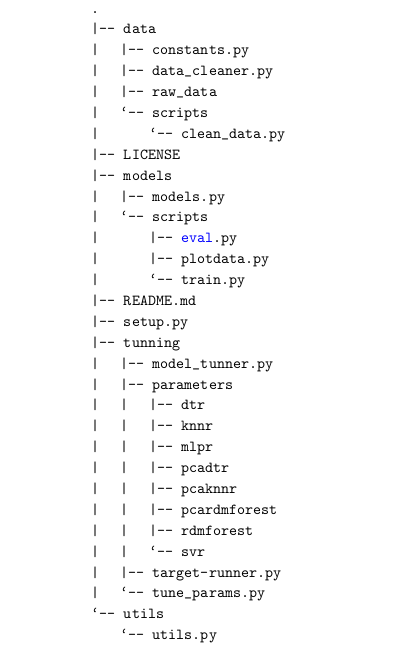
\includegraphics[width=0.6\textwidth]{images/proyecto_modeling}%
  \caption{Sistema para el ajuste de parámetros y modelado}\label{fig:proyecto_modelado}
  \end{figure}

\end{appendix}

\addcontentsline{toc}{chapter}{\numberline{}Bibliografía}
\bibliographystyle{plaindin_esp}
\bibliography{BibliMSc}
\end{document}
